\subsection{Некоторые примеры}

На рис.~\ref{fig:xsec_2d} представлены дважды дифференциальные сечения $\frac{d^2\sigma}{dx\,dy}$ для взаимодействия мюонного нейтрино с протоном через обмен бозоном $W$, рассчитанные при различных энергиях нейтрино и фиксированных значениях переменной $y$. Характерной особенностью этих графиков является то, что с ростом энергии основная часть сечения смещается в область всё меньших значений переменной Бьёркена $x$. Это отражает фундаментальную особенность глубоко-неупругого рассеяния: при больших $Q^2$ всё больший вклад в сечение начинают вносить морские кварки и антикварки.

\begin{figure}[!h]
\centering
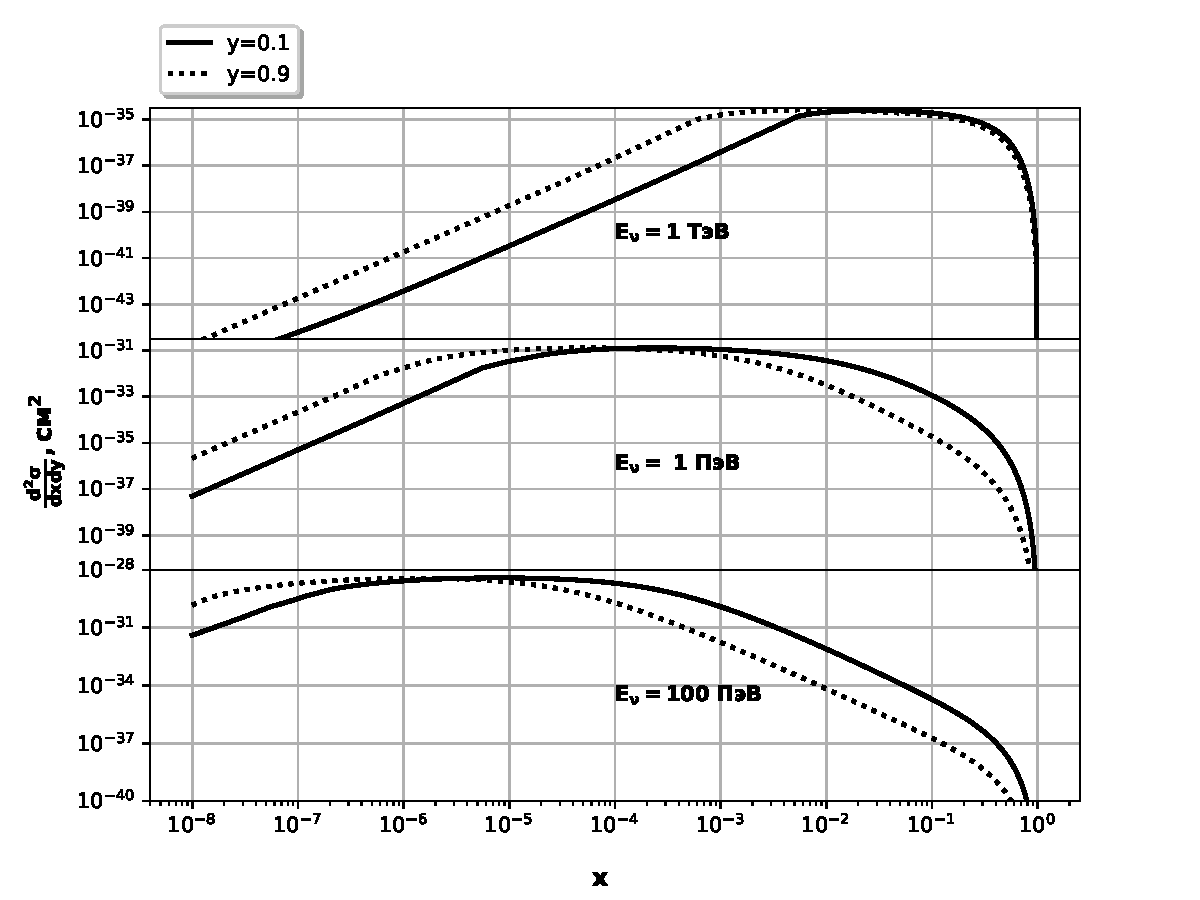
\includegraphics[width=\linewidth]{'images/NuProp/xs_vs_xCT18ZNNLO_cc_12_proton.pdf'}
\caption{Дважды дифференциальные сечения для рассеяния мюонного нейтрино на протоне за счёт заряженного тока в зависимости от переменной Бьёркена $x$ при различных энергиях нейтрино и фиксированных значениях переменной $y$.}
\label{fig:xsec_2d}
\end{figure}

На достаточно высоких энергиях нейтрино (\~ 0.1 ГэВ) достигается область $x \lesssim 10^{-5}$ и ниже, где партонные распределения плохо определены, поскольку соответствующие данные либо отсутствуют, либо экстраполированы из области $x \gtrsim 10^{-4}$. Это приводит к увеличению неопределённости в расчёте полного сечения, особенно при использовании различных наборов PDF.

Оценка вклада неизмеренного фазового пространства в общее сечение — одна из ключевых целей настоящей работы. На рис.~\ref{fig:xsec_total} показана зависимость полного сечения взаимодействия мюонного нейтрино на нуклоне от энергии для различных партонных распределений. Видно, что при $E_\nu \gtrsim 10^5$~ГэВ расчёты, основанные на разных PDF-наборах, начинают расходиться, отражая растущую модельную неопределённость в области малых $x$. Именно в этой области наш подход позволяет количественно оценить вклад недостоверно измеренных компонент, таких как морские кварки и глюоны, в предсказания полного сечения.


\begin{figure}[!h]
\centering
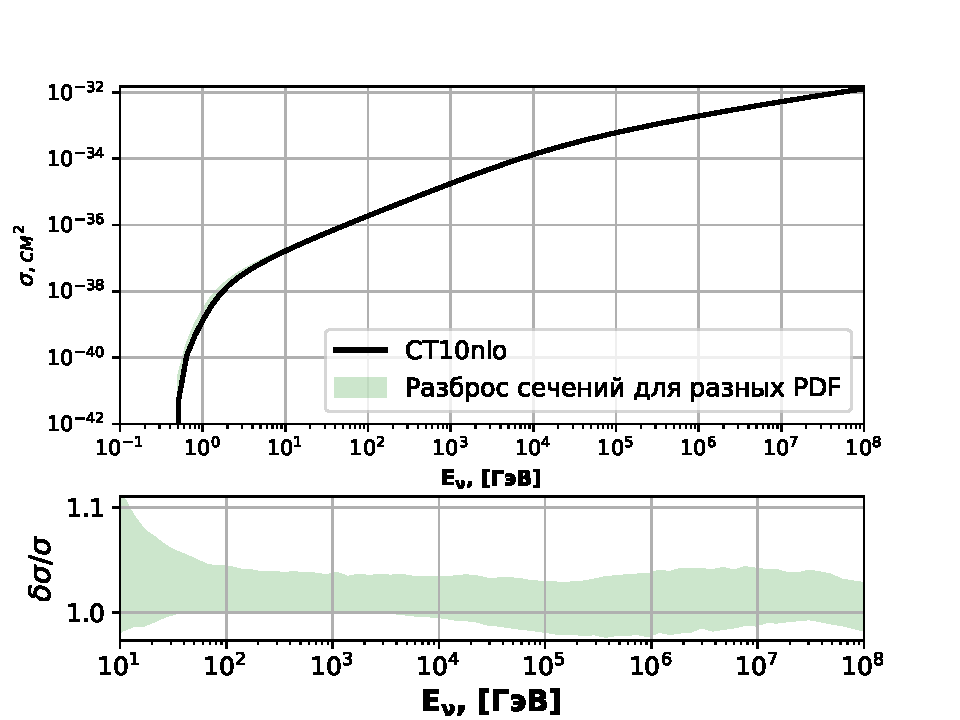
\includegraphics[width=\linewidth]{'images/NuProp/xs_vs_enu.pdf'}
\caption{Полные сечения взаимодействия мюонного нейтрино на нуклоне в зависимости от энергии $E_\nu$ для различных наборов партонных распределений (\texttt{CT18ZNNLO}, \texttt{nCTEQ15}, \texttt{CT10nlo}, \texttt{TUJU19_nlo}). Расхождение при высоких энергиях отражает неопределённость поведения PDF при малых $x$.} 
\label{fig:xsec_total}
\end{figure}
